\documentclass[../talk.tex]{subfiles}
\begin{document}

\begin{frame}{Compositional verification}
    \begin{overlayarea}{\slidewidth}{\slideheight}
        \begin{center}
                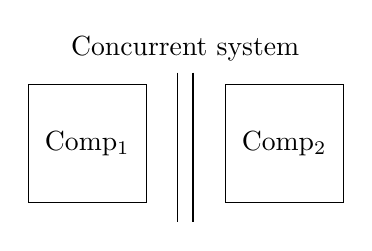
\begin{tikzpicture}

                    \node (comp1) at (0,0) [minimum width=1.5cm,minimum height=1.5cm, anchor=west,draw] {Comp$_1$};
                    \node (comp2) at (2.5,0) [minimum width=1.5cm,minimum height=1.5cm, anchor=west,draw] {Comp$_2$};

                    \node at (2,1.2) {Concurrent system};
                    \draw
                        (1.9,0.9) -- +(0,-1.9)
                        (2.1,0.9) -- +(0,-1.9)
                    ;
                \end{tikzpicture}
            \end{center}

            \only<1>%
            {%
                \alert{State explosion problem}

                    \begin{center}
                        % \(
                            \begin{tabular}{l@{}l@{}l@{}l@{}l}
                                $\#\text{LoC}(\text{Comp}_1 \!\mid\mid\! \text{Comp}_2)$
                                &\ $=$ \ &
                                $\#\text{LoC}(\text{Comp}_1)$
                                &\ $+$ \ &
                                $\#\text{LoC}(\text{Comp}_2)$
                                \\
                                %
                                    $\#\text{States}(\text{Comp}_1 \!\mid\mid\! \text{Comp}_2)$
                                    &\ $=$ \ &
                                    $\#\text{States}(\text{Comp}_1)$%
                                    &\ \alert{$*$}\ &
                                    $\#\text{States}(\text{Comp}_2)$
                                %
                            \end{tabular}
                        % \)
                    \end{center}


                \vspace*{1em}

                    Solution: \alert{Compositional verification}

                    \quad verify each component separately
            }
            \only<2>%
            {%
                \vspace*{-0.5em}
                \alert{Assume-guarantee reasoning} [Jones 1983]

                    \vspace*{-1em}
                    \[
                        \relyguarantee{\text{Assume}}{\text{Comp}}{\text{Guarantee}}
                        \text{ satisfied if}
                    \]
                        \(
                            \forall \text{Env} \colon \text{Comp} \!\mid\mid\! \text{Env} \models \text{Assume}
                            \implies
                            \text{Comp} \!\mid\mid\! \text{Env} \models \text{Guarantee}
                        \)


                    \vspace*{1em}

                    Asymmetric \alert{proof rule} for two components:

                    \begin{columns}[T]
                                \begin{column}{0.6\textwidth}
                                            \begin{tabular}{l}
                                                $\relyguarantee{\true}{\text{Comp}_1}{\text{Assume}}$
                                                \\
                                                $\relyguarantee{\text{Assume}}{\text{Comp}_2}{\text{Guarantee}}$
                                                \\
                                                \cline{1-1}
                                                $\relyguarantee{\true}{\text{Comp}_1 \!\mid\mid\! \text{Comp}_2 }{\text{Guarantee}}$
                                                \\
                                            \end{tabular}
                                        % \)
                                \end{column}
                                    \begin{column}{0.4\textwidth}
                                        When checking $\text{Comp}_2$:
                                        \begin{itemize}
                                            \item[] \alert{Environment}: $\text{Comp}_1$
                                            \item[] \alert{Certificate}: $\text{Assume}$
                                        \end{itemize}
                                    \end{column}
                            \end{columns}
            }
    \end{overlayarea}
\end{frame}

\end{document}
